\documentclass{beamer}
\usepackage{amsmath}
\usepackage{amssymb}
\usepackage{geometry}
\usepackage{graphicx}
\usepackage{url}
\usepackage{xcolor}

% some latex magic for correcting apostrophe issue in verbatim mode
\makeatletter
\let \@sverbatim \@verbatim
\def \@verbatim {\@sverbatim \verbatimplus}
{\catcode`'=13 \gdef \verbatimplus{\catcode`'=13 \chardef '=13 }} 
\makeatother

\begin{document}

%---------------------------------------------
\begin{frame}
\large
Lecture 5:\\
Normal Distribution\\
STAT 310, Spring 2021
\normalsize
\end{frame}

%----------------------------------------------
\begin{frame}
\begin{itemize}
\item The normal distribution is one of the most common and important probability distributions.
\vspace{5pt}
\item It is symmetric, unimodal, and bell-curve shaped.
\vspace{5pt}
\item Many phenomena in nature approximately follow a normal distribution such as the height of individuals, the velocity in any direction of a molecule of gas, and measurement error.
\end{itemize}
\begin{figure}
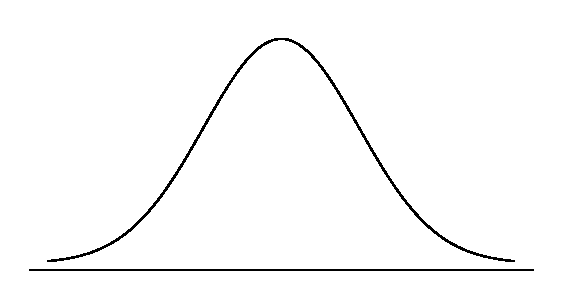
\includegraphics[scale=0.55]{figure/norm_draw}
\end{figure}
\end{frame}

%----------------------------------------------
\begin{frame}
\begin{itemize}
\item The normal distribution curve is a mathematical abstraction.
\vspace{5pt}
\item Just as there is no such thing as a perfect circle, no real data set perfectly follows a normal distribution.
\vspace{5pt}
\item However, many data sets \emph{approximately} follow a normal distribution, and so the normal distribution provides a very useful approximation for a variety of problems.
\end{itemize}
\end{frame}

%----------------------------------------------
\begin{frame}
\begin{figure}
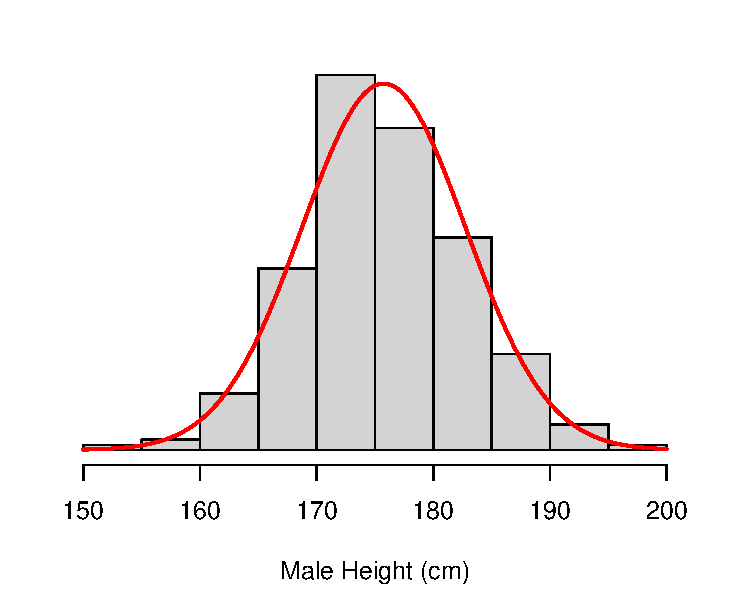
\includegraphics[scale = 0.5]{figure/height_hist_norm.pdf}
\caption{Histogram of male heights (cm) with normal distribution curve. We see that the distribution of height is approximately normal.}
\end{figure}
\end{frame}

%----------------------------------------------
% \begin{frame}
% ``As far as the laws of mathematics refer to reality, they are not certain; and as far as they are certain, they do not refer to reality." -- Albert Einstein\\
% \vspace{10pt}
% ``All models are wrong, but some are useful." -- George Box
% % add pictures
% \end{frame}
% no model or mathematical law is a perfect description, but they are useful approximations

%----------------------------------------------
\begin{frame}
\begin{itemize}
\item The normal distribution is characterized by two parameters: the mean, $\mu$, and standard deviation, $\sigma$.
\vspace{5pt}
\item The mean specifies the center of the distribution.  Changing the value of the mean shifts the bell-curve to the left or right.
\vspace{5pt}
\item The standard deviation specifies the spread of the distribution.  Changing the value of the standard deviation stretches or constricts the bell-curve.
\end{itemize}
\end{frame}

%----------------------------------------------
\begin{frame}
\begin{itemize}
%\item Informally, by ``random variable", we mean a variable that takes on values which represents outcomes of a random process, such as a person's weight or daily temperature.  Usually random variables are denoted with upper-case letters.
\item The notation $X \sim N(\mu, \sigma)$ means that the random variable $X$ follows a normal distribution with mean $\mu$ and standard deviation $\sigma$.
\vspace{5pt}
\item For example, the plot below shows the distribution of $N(\mu = 10, \sigma = 3)$
\end{itemize}
\begin{figure}
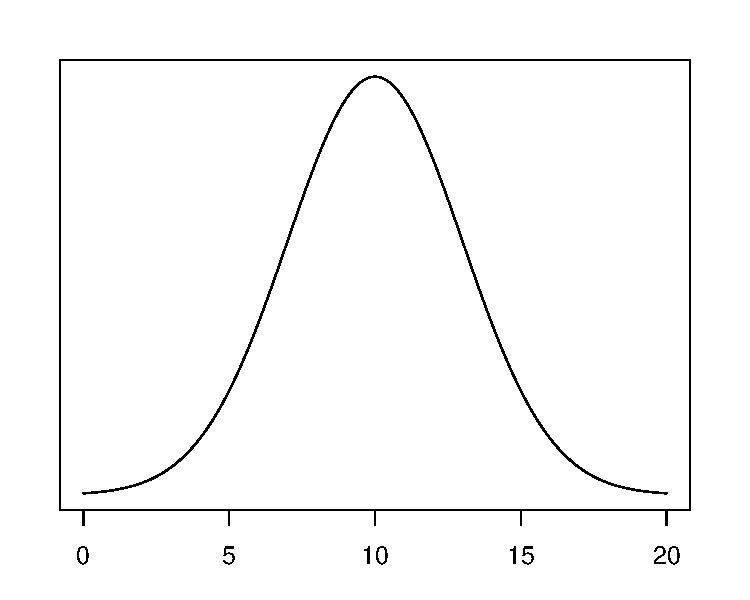
\includegraphics[scale=0.3]{figure/norm1.pdf}
\end{figure}
\end{frame}

\begin{frame}
\begin{figure}
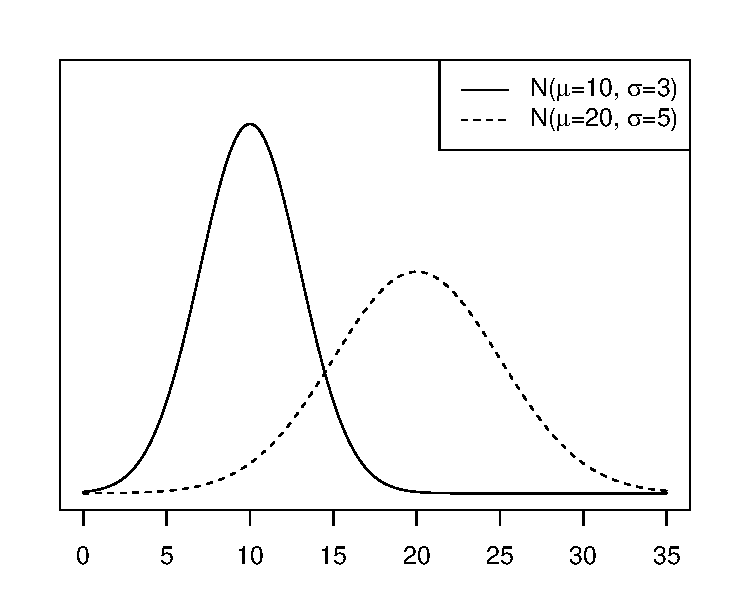
\includegraphics[scale=0.65]{figure/norm2.pdf}
\caption{Plot of two normal distributions.}
\end{figure}
\end{frame}

%----------------------------------------------
\begin{frame}
\begin{itemize}
\item Probabilities are computed as the area under the normal distribution curve.
\vspace{5pt}
\item The total area under the normal distribution curve is always 1.
\end{itemize}
\begin{figure}
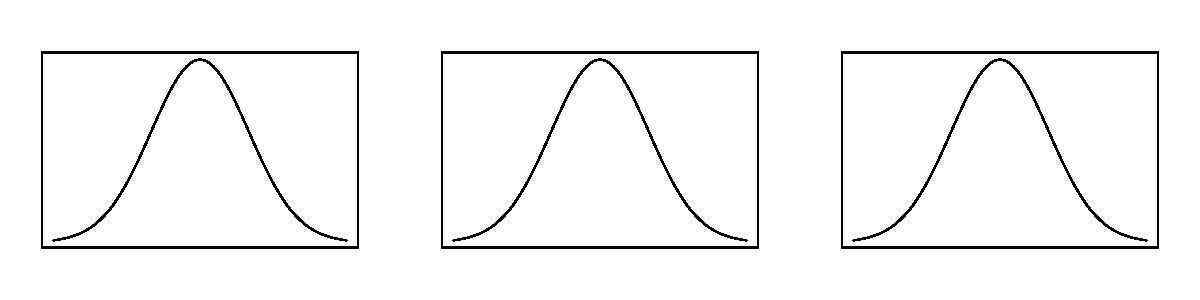
\includegraphics[scale=0.55]{figure/norm3}
\end{figure}
\end{frame}

%----------------------------------------------
\begin{frame}{Empirical Rule}
\begin{figure}
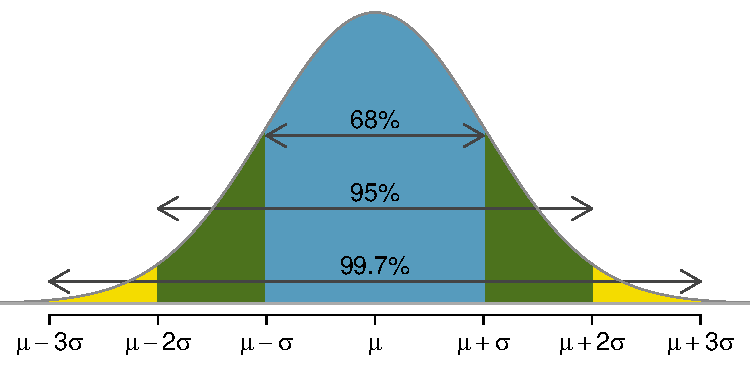
\includegraphics[scale=0.55]{figure/empirical.pdf}
\end{figure}
\small
\begin{itemize}
\item About 68\% of the distribution is contained within 1 standard deviation of the mean.
\item About 95\% of the distribution is contained within 2 standard deviations of the mean.
\item About 99.7\% of the distribution is contained within 3 standard deviations of the mean.
\end{itemize}
\end{frame}

\begin{frame}{Standardizing with z-scores}
\begin{itemize}
\item The normal distribution with mean $\mu = 0$ and standard deviation $\sigma = 1$ is called the \textbf{standard normal distribution} or \textbf{Z-distribution}.
\vspace{5pt}
\item If $x$ is an observation from $N(\mu, \sigma)$, we define the $z$-score as
$$z = \frac{x - \mu}{\sigma}$$
% \item Computing $Z$-scores allows us to compute probabilities for any normal distribution by either using the standard normal table or the R function \texttt{pnorm()}.
\end{itemize}
\end{frame}

\begin{frame}{Standardizing with z-scores}
\begin{itemize}
\item A $z$-score can be interpreted as the number of standard deviations an observation $x$ lies away from the mean.
\vspace{5pt}
\begin{itemize}
\item For instance, if a student has a $z$-score of 2 on an exam then that student is 2 standard deviations \emph{above} the average score.
\vspace{5pt}
\item If a student has a $z$-score of -1.5 on an exam then that student is 1.5 standard deviations \emph{below} the average score.
\end{itemize}
\end{itemize}
\end{frame}

\begin{frame}{Example 1}
The SAT score $X$ of a students is normally distributed with mean $\mu=1100$ and standard deviation $\sigma = 200$. 
\begin{enumerate}[(a)]
\item Calculate and interpret the z-score for a student that scored a 1350 on the SAT.
\vspace{2.25cm}
\item Calculate and interpret the z-score for a student that scored a 900 on the SAT.
\vspace{2.25cm}
\end{enumerate}
\end{frame}

\begin{frame}{Example 2}
\vspace{-1.75cm}
\small
The amount $X$ of the pollutant nitrogen oxide in automobiles is normally distributed with mean $\mu=70$ ppb (parts per billion) and standard deviation $\sigma = 13$ ppb.  That is, $X \sim N(\mu = 70, \sigma = 13)$.
\begin{enumerate}[(a)]
\item What is the probability that a randomly selected vehicle will have an emission level less than 60 ppb?
\end{enumerate}
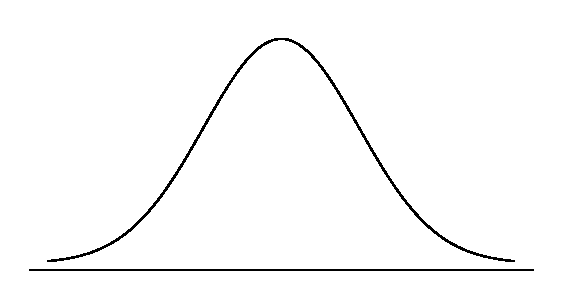
\includegraphics[scale=0.5]{figure/norm_draw.pdf}
\end{frame}

\begin{frame}{Example 2}
\vspace{-1.75cm}
\small
The amount $X$ of the pollutant nitrogen oxide in automobiles is normally distributed with mean $\mu=70$ ppb (parts per billion) and standard deviation $\sigma = 13$ ppb.  That is, $X \sim N(\mu = 70, \sigma = 13)$.
\begin{enumerate}[(b)]
\item What is the probability that a randomly selected vehicle will have an emission level greater than 90 ppb?
\end{enumerate}
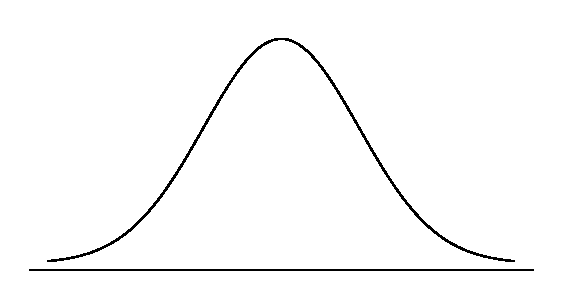
\includegraphics[scale=0.5]{figure/norm_draw.pdf}
\end{frame}

\begin{frame}{Example 2}
\vspace{-1.75cm}
\small
The amount $X$ of the pollutant nitrogen oxide in automobiles is normally distributed with mean $\mu=70$ ppb (parts per billion) and standard deviation $\sigma = 13$ ppb.  That is, $X \sim N(\mu = 70, \sigma = 13)$.
\begin{enumerate}[(c)]
\item What is the probability that a randomly selected vehicle will have an emission level between 60 and 90 ppb?
\end{enumerate}
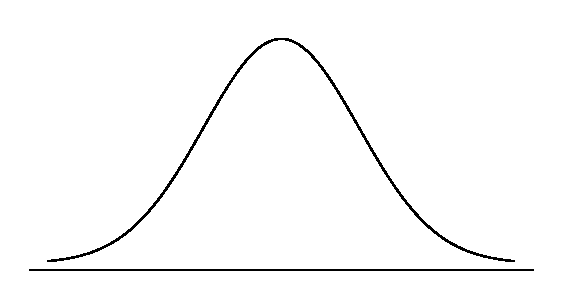
\includegraphics[scale=0.5]{figure/norm_draw.pdf}
\end{frame}

\begin{frame}{Example 3}
\vspace{-1.75cm}
\small
Body temperatures are normally distributed with mean $\mu=98.2$ and standard deviation $\sigma= 0.74$, in degrees Fahrenheit.\\  That is, $X \sim N(98.2, 0.74)$.
\begin{enumerate}[(a)]
\item Find the cutoff for the lowest 5\% of body temperatures (the $5^{th}$ percentile)?
\end{enumerate}
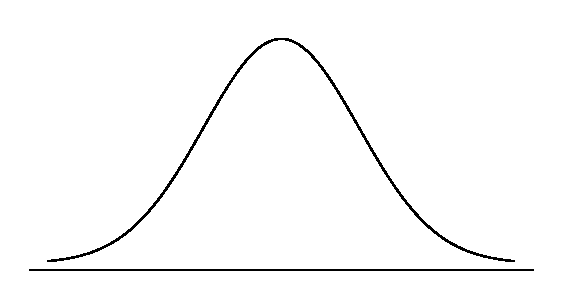
\includegraphics[scale=0.5]{figure/norm_draw.pdf}
\end{frame}

\begin{frame}{Example 3}
\vspace{-1.75cm}
\small
Body temperatures are normally distributed with mean $\mu=98.2$ and standard deviation $\sigma= 0.74$, in degrees Fahrenheit.  That is, $X \sim N(98.2, 0.74)$.
\begin{enumerate}[(b)]
\item Find the cutoff for the highest 15\% of body temperatures (the 85$^{th}$ percentile)?
\end{enumerate}
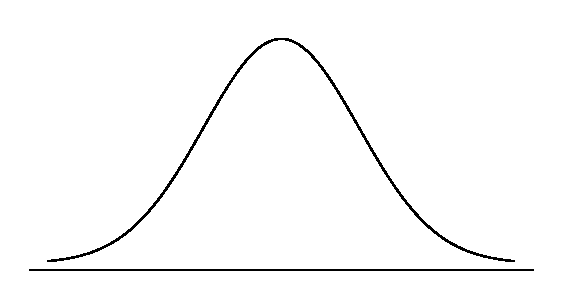
\includegraphics[scale=0.5]{figure/norm_draw.pdf}
\end{frame}



\end{document}